\documentclass[12pt]{article}
\usepackage{light}
\usepackage{verbatim}
\usepackage{graphicx}

\hidesolutions
%\showsolutions

%%%%% some macros needed %%%%%%%%%%%
%\newcommand{\eqdef}{\mathbin{::=}}
\newcommand{\mfigure}[3]{\bigskip\centerline{\resizebox{#1}{#2}{\includegraphics{#3}}}\bigskip}
\newcommand{\edge}[2]{\{#1\text{,}#2\}}
%\newcommand{\arc}[2]{#1\!\longrightarrow\!#2}
%\newcommand{\beqn}{\begin{eqnarray*}}
%\newcommand{\eeqn}{\end{eqnarray*}}
%\newcommand{\ok}{\marginpar{ok?}}
%%%%%%%%%%%%%%%%%%%%%%%%%%%%%%%%%%%%%

\begin{document}

\recitation{9}{October 12, 2016}


\section{Getting around a graph}

\begin{definition}\label{def:undirected-path}
A \term{walk}\footnote{Some texts use the word \emph{path} for our
  definition of walk and the term \emph{simple path} for our
  definition of path.} in a graph, $G$, is a sequence of vertices
\begin{equation*}
v_0, v_1, \dots, v_k
\end{equation*}
and edges
\begin{equation*}
    \edge{v_0}{v_1}, \edge{v_1}{v_2}, \dots, \edge{v_{k - 1}}{v_k}
\end{equation*} 
such that $\edge{v_i}{v_{i+1}}$ is an edge of $G$ for all $i$ where $0
\leq i < k$ .  The walk is said to \index{start of path}\emph{start}
at $v_0$ and to \index{end of walk}\emph{end} at $v_k$, and the
\index{length of walk}\emph{length} of the walk is defined to be $k$.
An edge, $\edge{u}{v}$, is \term{traversed} $n$ times by the walk if
there are $n$ different values of $i$ such that $\edge{v_i}{v_{i+1}} =
\edge{u}{v}$.  
\end{definition}
\begin{definition}
A \term{path} is a walk where all the $v_i$'s are
different, that is, $i\neq j$ implies $v_i \neq v_j$.  For simplicity,
we will refer to paths and walks by the sequence of
vertices.\footnote{This works fine for simple graphs since the edges
  in a walk are completely determined by the sequence of vertices and
  there is no ambiguity.  For graphs with multiple edges, we would
  need to specify the edges as well as the nodes.}
\end{definition}

\begin{figure}[!h]

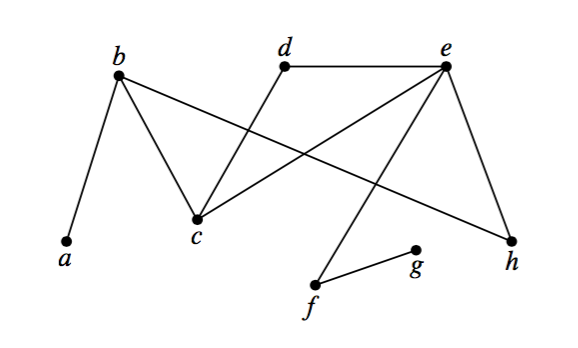
\includegraphics{distance-graph}
\centering
\caption{A graph containing a path $a$, $b$, $c$, $d$, $e$, $f$,~$g$
  of length~6.}
\label{dg}
\end{figure}

For example, the graph in Figure~\ref{dg} has a length~6 path $a$,
$b$, $c$, $d$, $e$, $f$,~$g$.  This is the longest path in the graph.
Of course, the graph has walks with arbitrarily large lengths; for
example, $a$, $b$, $a$, $b$, $a$, $b$,\,\dots.

The length of a walk or path is the total number of times it traverses
edges, which is \emph{one less} than its length as a sequence of
vertices.  For example, the length~6 path $a$, $b$, $c$, $d$, $e$,
$f$,~$g$ contains a sequence of 7~vertices.



\section*{Problem: Finding a Path}

Use the Well Ordering Principle to prove the following lemma.

\begin{lemma}\label{simplepath}
If there is a walk from a vertex $u$ to a vertex~$v$ in a graph, then
there is a path from $u$ to~$v$.
\end{lemma}

\solution{
\begin{proof}
Since there is a walk from $u$ to $v$, there must, by the
Well-ordering Principle, be a minimum length walk from $u$ to~$v$.  If
the minimum length is zero or one, this minimum length walk is itself
a path from $u$ to $v$.  Otherwise, there is a minimum length walk
\[
v_0, v_1, \dots, v_k
\]
from $u = v_0$ to $v = v_k$ where $k \geq 2$.  We claim this walk must
be a path.  To prove the claim, suppose to the contrary that the walk
is not a path; that is, some vertex on the walk occurs twice.  This
means that there are integers $i,j$ such that $0 \leq i < j \leq k$
with $v_i= v_j$.  Then deleting the subsequence
\[
    v_{i+1}, \dots, v_j
\]
yields a strictly shorter walk
\[
    v_0, v_1,\dots, v_i,v_{j+1},v_{j+2},\dots, v_k
\]
from $u$ to $v$, contradicting the minimality of the given walk.
\end{proof}

Actually, we proved something stronger:
\begin{corollary}\label{ss}
For any walk of length $k$ in a graph, there is a path of length
\emph{at most} $k$ with the same endpoints.  Moreover, the shortest
walk between a pair of vertices is, in fact, a path.
\end{corollary}
}


\section{Matrix Multiplication}
Although this may be a review for some, it will be an important part of tomorrow's lecture when we describe graphs using an \emph{adjacency matrix}.

Recall the definition of matrix multiplication. Given two matrices $A$ and $B$, where $A$ is $m \times n$ and $B$ is $n \times k$ their product is given by:


\begin{equation*}
A \cdot B =
\begin{bmatrix}
    a_{11} & a_{12} & \dots  & a_{1n} \\
    a_{21} & a_{22} & \dots  & a_{2n} \\
    \vdots & \vdots & \ddots & \vdots \\
    a_{m1} & a_{m2} & \dots  & a_{mn}
\end{bmatrix} \cdot
\begin{bmatrix}
    b_{11} & b_{12} & \dots  & b_{1k} \\
    b_{21} & b_{22} & \dots  & b_{2k} \\
    \vdots & \vdots & \ddots & \vdots \\
    b_{n1} & b_{n2} & \dots  & b_{nk}
\end{bmatrix} =
\begin{bmatrix}
    c_{11} & c_{12} & \dots  & c_{1k} \\
    c_{21} & c_{22} & \dots  & c_{2k} \\
    \vdots & \vdots & \ddots & \vdots \\
    c_{m1} & c_{m2} & \dots  & c_{mk}
\end{bmatrix} = C
\end{equation*}
where
\begin{equation*}
c_{ij} = \sum_{p=1}^n a_{ip}b_{pj}
\end{equation*}
Note that $C$ is a $m \times k$ matrix. 

It is also important to note that in general $A \cdot B \neq B \cdot A$. In fact, this operation may not even be defined, since the row dimension of the first matrix must equal the column dimension of the second (above, $A$ has $n$ rows and $B$ has $n$ columns).

Multiplying a matrix and a vector is identical, noting that a column vector is simply a $n \times 1$ matrix. 

Let's do some examples. 

\section*{Problems: Matrix Multiplication Practice}
\begin{enumerate}
\item Evaluate the following expressions.
\begin{enumerate}

\item
\begin{equation*}
\begin{bmatrix}
\alpha & \rho \\
\beta & \sigma \\
\gamma & \tau \\
\end{bmatrix}\begin{bmatrix}
a & b & c \\
x & y & z
\end{bmatrix}
\end{equation*}

\solution{
\begin{equation*}
\begin{bmatrix}
\alpha a + \rho x & \alpha b + \rho y & \alpha c + \rho z \\
\beta a + \sigma x & \beta b + \sigma y & \beta c + \sigma z \\
\gamma a + \tau x & \gamma b + \tau y & \gamma c + \tau z
\end{bmatrix}
\end{equation*}
}

\item
\begin{equation*}
\begin{bmatrix}
a & b & c \\
x & y & z
\end{bmatrix} 
\begin{bmatrix}
\alpha & \rho \\
\beta & \sigma \\
\gamma & \tau \\
\end{bmatrix} 
\end{equation*}
\solution{
\begin{equation*}
\begin{bmatrix}
a\alpha + b\beta + c \gamma & a\rho + b\sigma + c \tau \\
x\alpha + y\beta + z \gamma & x\rho + y\sigma + z \tau \\
\end{bmatrix}
\end{equation*}
}

\item
\begin{equation*}
\begin{bmatrix}
a & b & c & d \\
w & x & y & z
\end{bmatrix} 
\begin{bmatrix}
\alpha & \rho \\
\beta & \sigma \\
\gamma & \tau \\
\end{bmatrix} 
\end{equation*}
\solution{This is not defined, since the first matrix is $2 \times 4$ and the second is $3 \times 2$}

\end{enumerate}

\item
Prove the following lemma:
\begin{lemma}
Let $b$ be a $m \times 1$ vector whose entries are nonnegative and sum to 1. Let $A$ be a $n \times m$ matrix whose entries are nonnegative and each column sums to one. Then, the product $c=Ab$ is a $n \times 1$ vector whose entries are nonnegative and sum to one.
\end{lemma}

\solution{
\begin{proof}

The $i^{th}$ entry $c_i = \sum_{j=1}^{m}A_{ij}b_j$ is nonnegative since each $A_{ij}$ and $b_j$ is nonnegative. 

The sum of the entries in $c$ is 
\[
\sum_{i=1}^{n}c_i 
= \sum_{i=1}^{n}\sum_{j=1}^{m}A_{ij}b_j  
= \sum_{j=1}^{m}\sum_{i=1}^{n}A_{ij}b_j  \\
= \sum_{j=1}^{m}b_j\sum_{i=1}^{n}A_{ij} \\
= \sum_{j=1}^{m}b_j \\
= 1
\]
Where we used in the second to last equality the fact that the sum of every column in $A$ is 1, and in the final equality the fact that the sum of the entries in $b$ is 1.



\end{proof}
}

\end{enumerate}


\iffalse
\section{Problem: Build-up error}
Recall a graph is \term{connected} iff there is a path between every pair of its vertices.

\begin{falseclm*}
If every vertex in a graph has positive degree, then the graph is
connected.
\end{falseclm*}

\begin{enumerate}[(a)]

\item Prove that this Claim is indeed false by providing a
counterexample.

\solution{
There are many counterexamples; here is one:

\begin{figure}[!h]
\centering
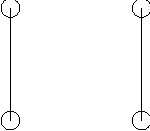
\includegraphics[scale = 0.75]{false-connect-cx}
\end{figure}
}

\item Since the Claim is false, there must be a logical mistake in the
following bogus proof.  Pinpoint the \emph{first} logical mistake
(unjustified step) in the proof.

\begin{proof}
  We prove the Claim above by induction.  Let $P(n)$ be the proposition
  that if every vertex in an $n$-vertex graph has positive degree, then
  the graph is connected.

\textbf{Base cases}: ($n \leq 2$).  In a graph with 1 vertex, that vertex
cannot have positive degree, so $P(1)$ holds vacuously.

$P(2)$ holds because there is only one graph with two vertices of positive
degree, namely, the graph with an edge between the vertices, and this
graph is connected.

\textbf{Inductive step}: We must show that $P(n)$ implies
$P(n+1)$ for all $n \geq 2$.  Consider an $n$-vertex graph in which every
vertex has positive degree.  By the assumption $P(n)$, this graph is
connected; that is, there is a path between every pair of vertices.  Now
we add one more vertex $x$ to obtain an $(n+1)$-vertex graph:

\mfigure{!}{1.75in}{false-connect-pic}

All that remains is to check that there is a path from $x$ to every other
vertex $z$.  Since $x$ has positive degree, there is an edge from $x$ to
some other vertex, $y$.  Thus, we can obtain a path from $x$ to $z$
by going from $x$ to $y$ and then following the path from $y$ to $z$.  This
proves $P(n+1)$.

By the principle of induction, $P(n)$ is true for all $n \geq 0$, which
proves the Claim.

\end{proof}

\solution{
This one is tricky: the proof is actually a good proof of
something else.  The first error in the proof is only in the final
statement of the inductive step: ``This proves $P(n+1)$''.

What we have actually shown (above) is that there are graphs on n+1 vertices
where each vertex has positive degree, and are connected. But if we want to
show that every graph on n+1 vertices where each vertex has positive
degree, is
necessarily connected, when we start with G and try to remove a node and all
edges incident to it we do not necessarily get a graph on n vertices that
satisfies the conditions we want. To put it more succinctly, in the
counterexample to part (a) every vertex we choose to delete results in a graph
where some node has degree zero afterwards.

\noindent \textit{Inductive step:} We must show that $P(n)$ implies
$P(n+1)$ for all $n \geq 1$.  Consider an $(n+1)$-vertex graph $G$ in
which every vertex has degree at least 1.  Remove an arbitrary vertex
$v$, leaving an $n$-vertex graph $G'$ in which every vertex has
degree... uh-oh!

The reduced graph $G'$ might contain a vertex of degree 0, making the
inductive hypothesis $P(n)$ inapplicable!  We are stuck--- and
properly so, since the claim is false!
}

\end{enumerate}

\fi

\section{Problem: Connectivity}

Prove that any simple graph with $n$ nodes and strictly more than $\tfrac12(n-1)(n-2)$ edges is connected.
%\emph{(Hint: try to prove the equivalent statement that any disconnected graph on $n$ nodes has at most $(n-1)(n-2)/2$ edges.}
\solution{
    We'll show the equivalent statement that any disconnected graph on $n$ nodes has at most $(n-1)(n-2)/2$ edges.

    Let $G=(V,E)$ be any graph on $n$ nodes that is not connected. Then there must be more than one connected component; let $G_1 = (V_1, E_1)$ be any connected component, and let $G_2 = (V_2, E_2)$ be the graph induced on $V_2 := V - V_1$. 
    Note that there are no edges going between $G_1$ and $G_2$, and so $E_1 \cup E_2 = E$.

    How many edges can $G_1$ have? At most ${|V_1| \choose 2}$ edges (one for each pair of nodes). Similarly, $G_2$ can have at most ${|V_2| \choose 2}$ edges. 

    Write $t := |V_1|$; then $|V_2| = |V| - |V_1| = n - t$.
    So the total number of edges in $G$ is at most
    \[ \frac{t(t-1)}{2} + \frac{(n-t)(n-t-1)}{2}. \]
    If we simplify this, we get
    \[ |E| \leq \frac{n(n-1)}{2} - t(n-t). \]
    But since $1 \leq t \leq n-1$, $t(n-t) \geq n-1$. (You can confirm this with some calculus; it might help to draw $t(n-t)$ as a function of $t$; it's just a parabola.) So 
    \[ |E| \leq \frac{n(n-1)}{2} - (n-1) = \frac{(n-2)(n-1)}{2}. \]
}
\end{document}
